\chapter{Stabilità e Criterio di Nyquist}
\label{ch:nyquist}

In questo capitolo si affronta lo studio sistematico della \textbf{stabilità} negli amplificatori reazionati e nei sistemi dinamici lineari tempo-invarianti (LTI). La stabilità è la proprietà fondamentale che garantisce che un sistema, in risposta a una perturbazione di durata finita o al rumore, ritorni spontaneamente nel proprio punto di equilibrio senza entrare in oscillazione incontrollata o saturazione non lineare.

\section{Criteri di stabilità di un amplificatore}

Consideriamo il modello generale di un amplificatore con reazione (feedback), in cui il segnale d'ingresso $X_S(s)$ viene confrontato con il segnale di retroazione generato dal blocco $\beta(s)$:

\begin{figure}[H]
\centering
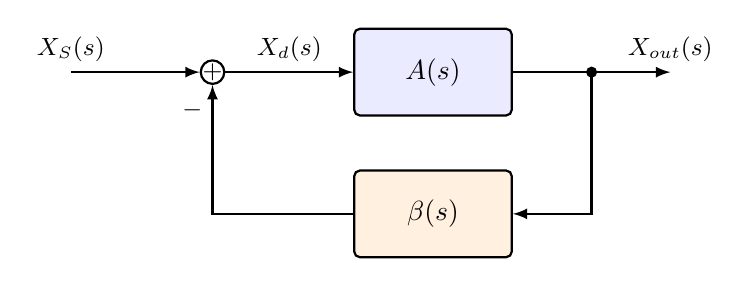
\begin{tikzpicture}[>=latex, font=\sffamily, scale=1.0]
    % Nodo sommatore
    \node[draw, circle, inner sep=3pt, thick] (sum) at (0,0) {};
    \node[font=\small] at (0,0) {$+$};
    
    % Blocco di guadagno diretto A(s)
    \node[draw, thick, minimum width=2.0cm, minimum height=1.1cm, fill=blue!8, rounded corners=2pt] (A) at (2.8, 0) {$A(s)$};
    
    % Blocco di retroazione \beta(s)
    \node[draw, thick, minimum width=2.0cm, minimum height=1.1cm, fill=orange!12, rounded corners=2pt] (beta) at (2.8, -1.8) {$\beta(s)$};
    
    % Ingresso
    \draw[->, thick] (-1.8, 0) node[above, font=\small] {$X_S(s)$} -- (sum);
    
    % Connessione sommatore -> A(s)
    \draw[->, thick] (sum) -- node[above, font=\small] {$X_d(s)$} (A);
    
    % Connessione A(s) -> Uscita e nodo di diramazione
    \draw[->, thick] (A.east) -- ++(2.0, 0) coordinate (outnode) node[above, font=\small] {$X_{\text{out}}(s)$};
    \fill (outnode) ++(-1.0, 0) circle (2pt);
    
    % Ramo di retroazione verso \beta(s)
    \draw[->, thick] (outnode) ++(-1.0, 0) |- (beta.east);
    
    % Ramo di retroazione da \beta(s) al sommatore (segno meno)
    \draw[->, thick] (beta.west) -| (sum.south) node[left, pos=0.9, font=\small] {$-$};
\end{tikzpicture}
\caption{Schema a blocchi ideale di un amplificatore reazionato ad anello chiuso.}
\end{figure}

Il guadagno ad anello chiuso dell'amplificatore vale:
\[
    A_F(s) \equiv A_V(s) = \frac{A(s)}{1 + A(s)\beta(s)} = \frac{A(s)}{1 + L(s)}
\]
dove $L(s) = A(s)\beta(s)$ indica il \textbf{guadagno d'anello} (\emph{loop gain}).

\begin{important}
\textbf{Condizioni sul guadagno d'anello $A\beta$:}
\begin{itemize}
    \item $A\beta \le -1$: \textbf{condizione sufficiente per la non-linearità}. In questo regime il denominatore scompare o diventa negativo, portando il circuito in saturazione o in oscillazione permanente (\emph{circuito non lineare}).
    \item $A\beta > -1$: \textbf{condizione necessaria per la linearità}. Affinché un amplificatore funzioni come sistema lineare è indispensabile che $A\beta > -1$.
\end{itemize}
\end{important}

\subsection{1. Risposta alla perturbazione / rumore in assenza di segnale ($X_S = 0$)}

Un sistema si definisce \textbf{stabile} se, in assenza di segnale utile in ingresso ($X_S = 0$), una qualsiasi perturbazione o rumore aleatorio $X_n(t)$ produce una risposta temporale che si estingue transitoriamente per $t \to \infty$:
\[
    \textbf{Sistema Stabile} \iff \text{Risposta al rumore} = \text{Transitorio} \quad (X_{\text{out}}(t) \xrightarrow{t \to \infty} 0)
\]

\begin{figure}[H]
\centering
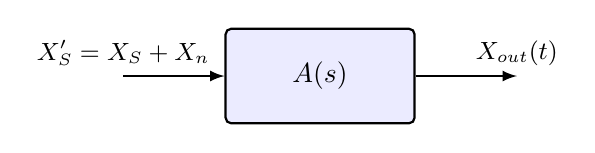
\begin{tikzpicture}[>=latex, font=\sffamily]
    \node[draw, thick, minimum width=2.4cm, minimum height=1.2cm, fill=blue!8, rounded corners=2pt] (A) at (0,0) {$A(s)$};
    \draw[->, thick] (-2.5,0) node[above, font=\small] {$X_S' = X_S + X_n$} -- (A);
    \draw[->, thick] (A) -- (2.5,0) node[above, font=\small] {$X_{\text{out}}(t)$};
\end{tikzpicture}
\caption{Modello di risposta alla perturbazione d'ingresso.}
\end{figure}

Sia il segnale totale d'ingresso $X_S'(t) = X_S(t) + X_n(t)$, dove $X_S$ è il segnale deterministico e $X_n$ è il rumore. Nel dominio di Laplace:
\[
    \tilde{X}_{\text{out}}'(s) = A(s) \tilde{X}_S'(s) = A(s) \tilde{X}_S(s) + A(s) \tilde{X}_n(s)
\]
In assenza di segnale ($X_S = 0$), la risposta temporale è la sola antitrasformata del rumore:
\[
    X_{\text{out}}'(t) = \mathcal{L}^{-1}\left\{ A(s) \tilde{X}_n(s) \right\} \xrightarrow{t \to \infty} 0
\]

\subsection{2. Risposta all'impulso ($\delta$ di Dirac)}

Un criterio equivalente e pratico richiede che la risposta a un impulso unitario (modello di perturbazione istantanea del tipo $\delta$ di Dirac) sia transitoria:
\[
    \textbf{Sistema Stabile} \iff \text{Risposta all'impulso } \delta(t) = \text{Transitorio} \quad (h(t) \xrightarrow{t \to \infty} 0)
\]
Se il rumore è modellato come impulso $\delta(t)$, con $\mathcal{L}\{\delta(t)\} = 1$, la risposta spettrale è $\tilde{X}_{\text{out}}(s) = A(s)$. Pertanto:
\[
    X_{\text{out}}(t) = \mathcal{L}^{-1}\{ A(s) \} \xrightarrow{t \to \infty} 0
\]

\subsection{Analisi dei poli e condizione di stabilità nel dominio di Laplace}

Esprimiamo la funzione di trasferimento come rapporto di polinomi fattorizzati in zeri $z_i$ e poli $p_k$:
\[
    A(s) = \frac{N(s)}{D(s)} = K \frac{\prod_{i=1}^{M} (s - z_i)^{\alpha_i}}{\prod_{k=1}^{N} (s - p_k)^{\beta_k}} \qquad (\text{con } \text{deg } N \le \text{deg } D)
\]
dove $\beta_k$ rappresenta la molteplicità del polo $p_k$.

\begin{teorema}{Teorema di Traslazione sulle Frequenze}
\[
    \mathcal{L}\left\{ e^{pt} f(t) \right\} = \int_0^{+\infty} e^{pt} f(t) e^{-st} \, dt = \int_0^{+\infty} f(t) e^{-(s-p)t} \, dt = \tilde{f}(s-p)
\]
\end{teorema}

Integrando $n$-volte per parti e applicando il Teorema di Traslazione, l'antitrasformata del generico termine polare con molteplicità $\beta_k$ vale:
\[
    \mathcal{L}^{-1}\left\{ \frac{1}{(s - p_k)^{\beta_k}} \right\} = \frac{t^{\beta_k - 1}}{(\beta_k - 1)!} \, e^{p_k t}
\]
La risposta impulsiva nel tempo $X_{\text{out}}(t) = \mathcal{L}^{-1}\{A(s)\}$ si scrive dunque come combinazione lineare dei modi propri del sistema:
\[
    X_{\text{out}}(t) = \sum_{k} a_k \, \frac{t^{\beta_k - 1}}{(\beta_k - 1)!} \, e^{p_k t}
\]
Esprimendo ciascun polo in forma complessa $p_k = \text{Re}(p_k) + j \text{Im}(p_k)$:
\[
    e^{p_k t} = e^{\text{Re}(p_k) t} \cdot e^{j \text{Im}(p_k) t} = e^{\text{Re}(p_k) t} \left[ \cos(\text{Im}(p_k) t) + j \sin(\text{Im}(p_k) t) \right]
\]

\begin{teorema}{Criterio dei Poli per la Stabilità}
\begin{itemize}
    \item Se $\text{Re}(p_k) < 0 \,\, \forall k$: l'esponenziale smorzante $e^{\text{Re}(p_k) t} \to 0$ vince su qualsiasi potenza polinomiale per $t \to \infty$, garantendo $X_{\text{out}}(t) \to 0$. Il sistema è \textbf{STABILE}.
    \item Se anche solo un polo ha $\text{Re}(p_k) \ge 0$: la risposta divergerà o oscillerà indefinitamente per $t \to \infty$. Il sistema è \textbf{INSTABILE}.
\end{itemize}
\[
    \boxed{\textbf{Sistema Stabile} \iff \text{Re}(p_k) < 0 \quad \forall k \quad (\text{tutti i poli nel semipiano sinistro LHP})}
\]
\end{teorema}

\section{Stabilità negli amplificatori reazionati e risposta in frequenza}

Nel contesto degli amplificatori reazionati, il legame tra il segnale di ingresso $\tilde{X}_S(s)$ e il segnale di uscita $\tilde{X}_{\text{out}}(s)$ è governato dalla funzione di trasferimento ad anello chiuso $A_F(s)$:
\[
    \tilde{X}_{\text{out}}(s) = A_F(s) \tilde{X}_S(s) \qquad \text{dove} \quad A_F(s) = \frac{A(s)}{1 \pm \beta(s) A(s)} = \frac{A(s)}{1 \pm L(s)}
\]
in cui le componenti dell'anello di reazione sono definite come segue:
\begin{itemize}
    \item $+\beta > 0$: \textbf{feedback negativo} (reazione negativa, ad azione stabilizzante).
    \item $-\beta < 0$: \textbf{feedback positivo} (reazione positiva, ad azione instabilizzante).
    \item $A(s)$: \textbf{guadagno ad anello aperto} (amplificazione dello stadio principale).
    \item $\beta(s)$: \textbf{fattore di retroazione} (frazione del segnale di uscita riportata al nodo sommatore d'ingresso).
    \item $L(s) = \beta(s) A(s)$: \textbf{guadagno d'anello} (\emph{loop gain}), rappresenta il guadagno complessivo subito da un segnale dopo aver compiuto un giro completo dell'anello.
    \item $A_F(s)$: \textbf{guadagno ad anello chiuso}, rappresenta il comportamento complessivo del circuito reazionato e costituisce la funzione di trasferimento da studiare per determinarne la stabilità.
\end{itemize}

\begin{important}
\textbf{Relazione tra i poli di $A_F(s)$ e le radici dell'anello:}
\[
    \text{Poli di } A_F(s) \subseteq \left\{ \text{Poli di } A(s) \right\} \cup \left\{ \text{Zeri di } [1 \pm \beta(s)A(s)] \right\}
\]
(i poli di $A$ compaiono anche nel denominatore $1\pm\beta A$ e di norma si semplificano: i poli ``nuovi'' introdotti dalla reazione sono gli zeri di $1\pm\beta A$). L'amplificatore reazionato è \textbf{stabile} se e solo se $A_F(s)$ possiede \textbf{esclusivamente poli con parte reale strettamente negativa} ($\text{Re}(p) < 0$).
\end{important}

\subsection{Esistenza della risposta in frequenza e legame con Fourier}

Se l'amplificatore ad anello chiuso è stabile, la regione di convergenza della sua trasformata di Laplace racchiude l'asse immaginario del piano complesso ($s = j\omega$). Di conseguenza, è ben definita la risposta in frequenza $\hat{A}(\omega)$ ottenibile come restrizione della trasformata di Laplace alla sola retta $s = j\omega$:
\[
    \exists \, \mathcal{F}\{A(t)\} = \hat{A}(\omega) = \tilde{A}(j\omega) = \left. \mathcal{L}\{A(t)\} \right|_{s = j\omega}
\]
L'andamento della risposta in frequenza $A(j\omega)$ viene analizzato in maniera asintotica tramite i \textbf{diagrammi di Bode}, esprimendo la funzione di trasferimento nella forma polare:
\[
    A(j\omega) = K \frac{\prod_{i=1}^{M} (j\omega - z_i)^{\alpha_i}}{\prod_{k=1}^{N} (j\omega - p_k)^{\beta_k}}
\]

\subsection{Diagrammi di Bode di ampiezza e di fase}

\textbf{1. Modulo in dB:}
\[
    |A(j\omega)| = |K| \frac{\prod_{i=1}^{M} |j\omega - z_i|^{\alpha_i}}{\prod_{k=1}^{N} |j\omega - p_k|^{\beta_k}}
\]
\[
    A_{\text{dB}}(\omega) = 20 \log_{10}|K| + 20 \sum_{i=1}^{M} \alpha_i \log_{10}|j\omega - z_i| - 20 \sum_{k=1}^{N} \beta_k \log_{10}|j\omega - p_k|
\]

\textbf{Caso di zeri e poli reali:}
Per ogni singolo termine $(j\omega - z)$, il modulo vale:
\[
    |j\omega - z| = \sqrt{\omega^2 + z^2} \approx \begin{cases} 
        |z| & \text{per } \omega \ll |z| \\[0.3em]
        \omega & \text{per } \omega \gg |z| 
    \end{cases}
\]
Di conseguenza, il contributo in ampiezza per $\omega \gg |z|$ aumenta linearmente nel grafico semilogaritmico con pendenza $+20\alpha$ dB/decade per uno zero di molteplicità $\alpha$, e diminuisce con pendenza $-20\alpha$ dB/decade per un polo di molteplicità $\alpha$.

\begin{figure}[H]
\centering
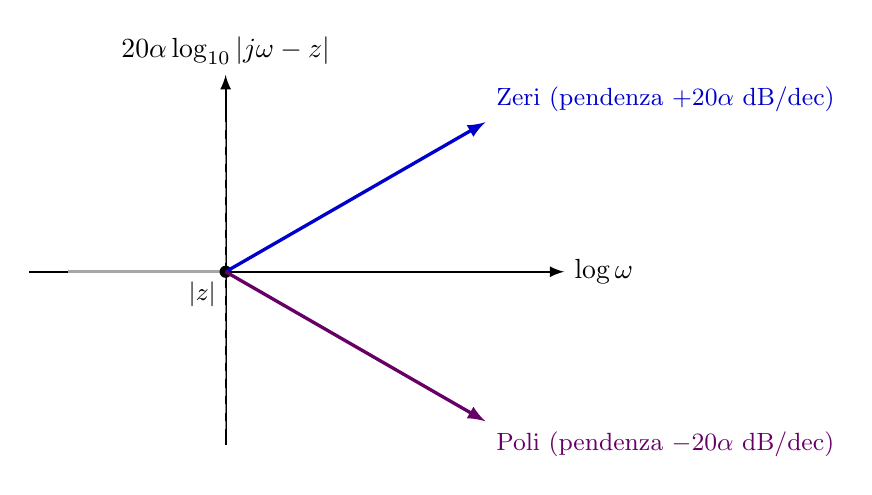
\begin{tikzpicture}[>=latex, font=\sffamily]
    % Assi
    \draw[->, thick] (0,0) -- (6.8,0) node[right] {$\log \omega$};
    \draw[->, thick] (2.5,-2.2) -- (2.5,2.5) node[above] {$20\alpha \log_{10}|j\omega - z|$};
    
    % Asintoto piatto
    \draw[very thick, gray!70] (0.5,0) -- (2.5,0);
    \draw[dashed, gray] (2.5,-2.0) -- (2.5,2.0);
    \node[below left, font=\small] at (2.5,0) {$|z|$};
    \fill (2.5,0) circle (2.2pt);
    
    % Asintoto Zero (+20\alpha dB/dec)
    \draw[very thick, blue!80!black, ->] (2.5,0) -- (5.8,1.9) node[above right, font=\small] {Zeri (pendenza $+20\alpha$ dB/dec)};
    
    % Asintoto Polo (-20\alpha dB/dec)
    \draw[very thick, violet!80!black, ->] (2.5,0) -- (5.8,-1.9) node[below right, font=\small] {Poli (pendenza $-20\alpha$ dB/dec)};
\end{tikzpicture}
\caption{Variazione asintotica della pendenza nel diagramma di ampiezza per zeri e poli reali di ordine $\alpha$.}
\end{figure}

\begin{important}
Attraversando uno zero o polo reale $\in \mathbb{R}$ di ordine $\alpha$, la pendenza del diagramma di Bode in ampiezza \textbf{aumenta} o \textbf{diminuisce} esattamente di $20\alpha$ dB/decade.
\end{important}

\textbf{2. Fase $\phi(\omega)$:}
\[
    \phi(\omega) = \arg(K) + \sum_{i=1}^{M} \alpha_i \arg(j\omega - z_i) - \sum_{k=1}^{N} \beta_k \arg(j\omega - p_k)
\]
L'andamento asintotico della fase rispetta le seguenti proprietà:
\begin{itemize}
    \item \textbf{Zeri generici} ($z \in \mathbb{R}$):
    \[
        \arg(j\omega - z) \simeq \begin{cases} 
            \arg(-z) = \begin{cases} 0 & \text{se } z < 0 \\ \pi & \text{se } z > 0 \end{cases} & \text{per } \omega \ll |z| \\[0.8em]
            \arg(j\omega) = +\dfrac{\pi}{2} & \text{per } \omega \gg |z| 
        \end{cases}
    \]
    \item \textbf{Poli reali stabili} ($p < 0$, poiché i poli devono trovarsi nel semipiano negativo LHP):
    \[
        \arg(j\omega - p) = \arg(j\omega + |p|) \simeq \begin{cases} 
            0 & \text{per } \omega \ll |p| \\[0.3em]
            +\dfrac{\pi}{2} & \text{per } \omega \gg |p| 
        \end{cases}
    \]
\end{itemize}

\begin{important}
La fase aumenta o diminuisce di $\pi/2$ ($90^\circ$) attraversando uno zero con $\alpha=1$ a seconda che sia a parte reale negativa o positiva. In generale:
\[
    \Delta \phi_Z = \pm \alpha \frac{\pi}{2} \quad (\text{con } z \lessgtr 0, \, \alpha \in \mathbb{N}) \qquad \qquad \Delta \phi_P = -\beta \frac{\pi}{2} \quad (\text{con } p < 0, \, \beta \in \mathbb{N})
\]
\end{important}

\subsection{Esempi canonici: Filtri Passa-basso, Passa-alto e Passa-banda}

Di seguito sono riportati i diagrammi di Bode asintotici e i relativi raccordi continui $C^\infty$ per le risposte filtro fondamentali.

\begin{figure}[H]
\centering

\begin{minipage}{0.48\textwidth}
\centering
\textbf{Passa-basso}\\[2ex]
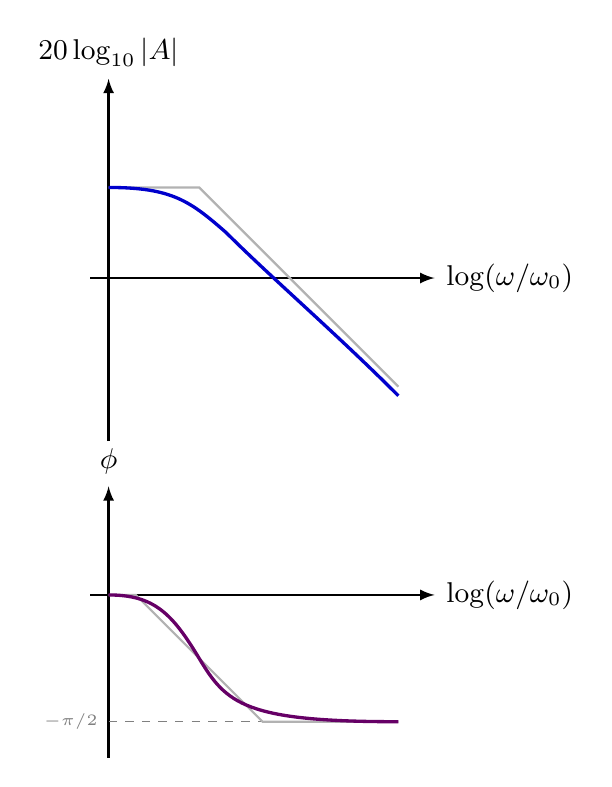
\begin{tikzpicture}[scale=1.15, transform shape, >=latex, font=\sffamily]
    \draw[->, thick] (-0.2,0) -- (3.6,0) node[right, font=\small] {$\log(\omega/\omega_0)$};
    \draw[->, thick] (0,-1.8) -- (0,2.2) node[above, font=\small] {$20\log_{10}|A|$};
    
    % Asintoto ampiezza
    \draw[gray!60, thick] (0,1) -- (1,1) -- (3.2,-1.2);
    % Raccordo C^\infty ampiezza
    \draw[blue!80!black, very thick] (0,1) .. controls (0.7,1) and (0.9,0.85) .. (1.3,0.5) .. controls (1.8,0.0) and (2.5,-0.6) .. (3.2,-1.3);
    
    % Fase sotto
    \begin{scope}[shift={(0,-3.5)}]
        \draw[->, thick] (-0.2,0) -- (3.6,0) node[right, font=\small] {$\log(\omega/\omega_0)$};
        \draw[->, thick] (0,-1.8) -- (0,1.2) node[above, font=\small] {$\phi$};
        \draw[dashed, gray] (0,-1.4) node[left, font=\tiny] {$-\pi/2$} -- (3.2,-1.4);
        
        % Asintoto fase
        \draw[gray!60, thick] (0,0) -- (0.3,0) -- (1.7,-1.4) -- (3.2,-1.4);
        % Raccordo C^\infty fase
        \draw[violet!80!black, very thick] (0,0) .. controls (0.5,0) and (0.7,-0.2) .. (1,-0.7) .. controls (1.3,-1.2) and (1.5,-1.4) .. (3.2,-1.4);
    \end{scope}
\end{tikzpicture}
\end{minipage}
\hfill
\begin{minipage}{0.48\textwidth}
\centering
\textbf{Passa-alto}\\[2ex]
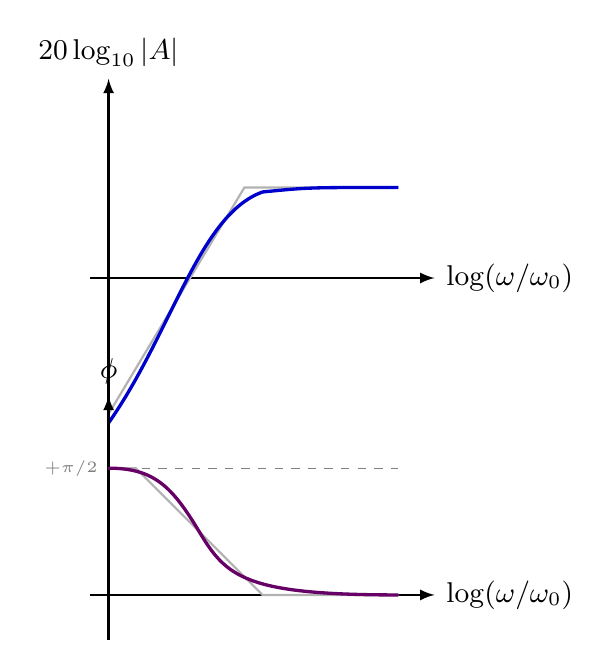
\begin{tikzpicture}[scale=1.15, transform shape, >=latex, font=\sffamily]
    \draw[->, thick] (-0.2,0) -- (3.6,0) node[right, font=\small] {$\log(\omega/\omega_0)$};
    \draw[->, thick] (0,-1.8) -- (0,2.2) node[above, font=\small] {$20\log_{10}|A|$};
    
    % Asintoto ampiezza
    \draw[gray!60, thick] (0,-1.5) -- (1.5,1) -- (3.2,1);
    % Raccordo C^\infty ampiezza
    \draw[blue!80!black, very thick] (0,-1.6) .. controls (0.7,-0.6) and (1.0,0.7) .. (1.7,0.95) .. controls (2.2,1) .. (3.2,1);
    
    % Fase sotto
    \begin{scope}[shift={(0,-3.5)}]
        \draw[->, thick] (-0.2,0) -- (3.6,0) node[right, font=\small] {$\log(\omega/\omega_0)$};
        \draw[->, thick] (0,-0.5) -- (0,2.2) node[above, font=\small] {$\phi$};
        \draw[dashed, gray] (0,1.4) node[left, font=\tiny] {$+\pi/2$} -- (3.2,1.4);
        
        % Asintoto fase
        \draw[gray!60, thick] (0,1.4) -- (0.3,1.4) -- (1.7,0) -- (3.2,0);
        % Raccordo C^\infty fase
        \draw[violet!80!black, very thick] (0,1.4) .. controls (0.5,1.4) and (0.7,1.2) .. (1,0.7) .. controls (1.3,0.2) and (1.5,0) .. (3.2,0);
    \end{scope}
\end{tikzpicture}
\end{minipage}

\vspace{1.5cm}

\begin{minipage}{\textwidth}
\centering
\textbf{Passa-banda ($\alpha$)}\\[2ex]
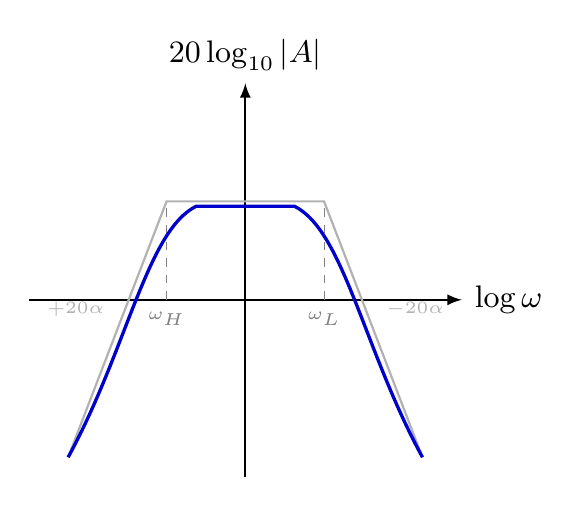
\begin{tikzpicture}[scale=1.25, transform shape, >=latex, font=\sffamily]
    \draw[->, thick] (-0.2,0) -- (4.2,0) node[right, font=\small] {$\log\omega$};
    \draw[->, thick] (2,-1.8) -- (2,2.2) node[above, font=\small] {$20\log_{10}|A|$};
    
    % Asintoti ampiezza
    \draw[gray!60, thick] (0.2,-1.6) -- node[above left, font=\tiny] {$+20\alpha$} (1.2,1) -- (2.8,1) -- node[above right, font=\tiny] {$-20\alpha$} (3.8,-1.6);
    \draw[dashed, gray] (1.2,0) node[below, font=\tiny] {$\omega_H$} -- (1.2,1);
    \draw[dashed, gray] (2.8,0) node[below, font=\tiny] {$\omega_L$} -- (2.8,1);
    
    % Raccordo C^\infty ampiezza
    \draw[blue!80!black, very thick] (0.2,-1.6) .. controls (0.8,-0.5) and (1.0,0.7) .. (1.5,0.95) -- (2.5,0.95) .. controls (3.0,0.7) and (3.2,-0.5) .. (3.8,-1.6);
\end{tikzpicture}
\end{minipage}

\caption{Diagrammi di Bode asintotici (grigio) e raccordi continui $C^\infty$ (blu/viola) per i filtri Passa-basso, Passa-alto e Passa-banda di ordine $\alpha$.}
\end{figure}

\begin{important}
\textbf{Riepilogo di zeri e poli per i filtri canonici ($RC = 1/\omega_0$):}
\begin{itemize}
    \item \textbf{Filtro passa-basso}: $A_{\text{LP}}(s) = \dfrac{1}{1 + sRC}$ con $K=1$, \textbf{zeri}: nessuno, \textbf{poli}: $s = -\omega_0$ ($\beta=1$).
    \item \textbf{Filtro passa-alto}: $A_{\text{HP}}(s) = \dfrac{sRC}{1 + sRC}$ con $K=1$, \textbf{zeri}: $s = 0$ ($\alpha=1$), \textbf{poli}: $s = -\omega_0$ ($\beta=1$).
    \item \textbf{Filtro passa-banda (ordine $\alpha$)}: $A_{\text{BP}}(s) = \dfrac{K s^\alpha}{(s + \omega_H)^\alpha (s + \omega_L)^\alpha}$, \textbf{zeri}: $s = 0$ ($\alpha$), \textbf{poli}: $s = -\omega_L, \, s = -\omega_H$ ($\alpha$).
\end{itemize}
\end{important}

\subsection{Esempio: Circuito sfasatore variabile (Filtro passa-tutto / All-Pass)}

Un'applicazione particolarmente interessante dei diagrammi di Bode è il \textbf{circuito sfasatore variabile} (\emph{All-Pass Filter}), capace di modificare la fase del segnale di ingresso senza alterarne l'ampiezza a qualsiasi frequenza.

\begin{figure}[H]
\centering
\begin{circuitikz}[american, transform shape, scale=1.1, thick]
    \draw (0,0) node[op amp] (opamp) {};
    
    % Ramo ingresso invertente (-)
    \draw (opamp.-) to[R, l_=$R'$, -*] ++(-2,0) coordinate (inM);
    
    % Ramo ingresso non-invertente (+)
    \draw (opamp.+) to[R, l_=$R$, -*] ++(-2,0) coordinate (inP);
    
    % Connessione tra i due rami in ingresso e generatore VS
    \draw (inM) -- (inP);
    \draw ($(inM)!0.5!(inP)$) to[short, *-o] ++(-1,0) node[left] {$V_S$};
    
    % Ramo di retroazione R'
    \draw (opamp.-) -- ++(0,1.5) coordinate (fb) to[R, l=$R'$] (fb -| opamp.out) -- (opamp.out);
    
    % Ramo condensatore verso massa
    \draw (opamp.+) -- ++(0,-1.5) to[C, l=$C$] ++(0,-1) node[ground] {};
    
    % Uscita Vout
    \draw (opamp.out) to[short, *-o] ++(1,0) node[right] {$V_{\text{out}}$};
\end{circuitikz}
\caption{Circuito sfasatore variabile (filtro passa-tutto).}
\end{figure}

Per sovrapposizione degli effetti o partitore d'ingresso, la tensione d'uscita vale:
\[
    V_{\text{out}} = V_S \left( \frac{2}{1 + sRC} - 1 \right) \implies A_V(s) = \frac{1 - sRC}{1 + sRC} = \frac{1 - s/\omega_0}{1 + s/\omega_0} \quad \left(\text{con } \omega_0 = \frac{1}{RC}\right)
\]
Analizzando la mappa zeri-poli nel piano complesso $s$:
\begin{itemize}
    \item \textbf{Zeri}: $s = +\omega_0 = +\frac{1}{RC}$ (zero a parte reale positiva RHP, $\alpha=1$).
    \item \textbf{Poli}: $s = -\omega_0 = -\frac{1}{RC}$ (polo a parte reale negativa LHP, $\beta=1$).
\end{itemize}

\textbf{Diagramma di Bode di modulo e fase:}
Nel dominio delle frequenze reali $s = j\omega$, il modulo vale $|A_V(j\omega)| = \frac{|1 - j\omega/\omega_0|}{|1 + j\omega/\omega_0|} = 1 \quad \forall \omega \implies 20\log_{10}|A_V| = 0\text{ dB}$.

\begin{figure}[H]
\centering
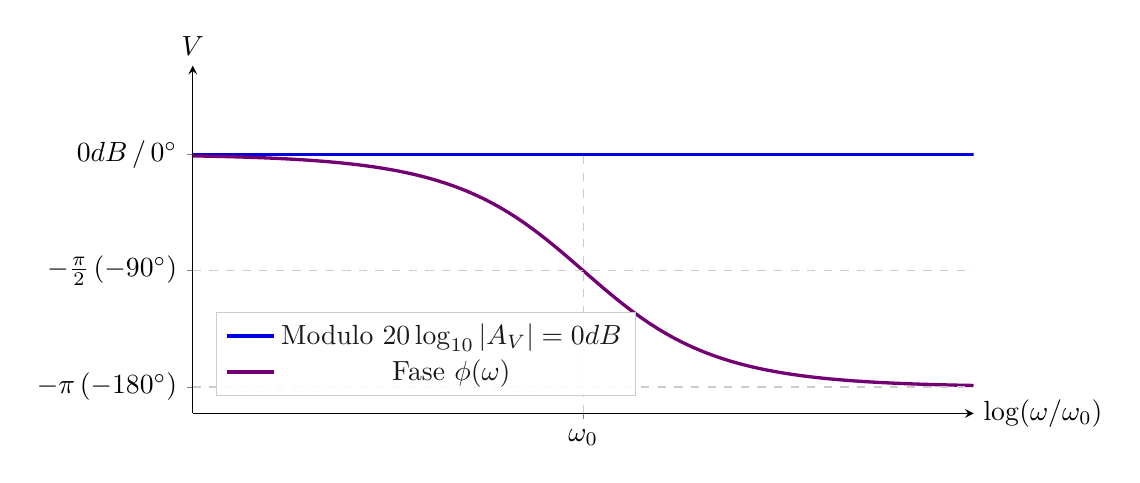
\begin{tikzpicture}
\begin{axis}[
    width=11.5cm, height=6.0cm,
    axis lines=left,
    xlabel={$\log(\omega/\omega_0)$},
    ylabel={$V$},
    xmin=-2, xmax=2,
    ymin=-3.5, ymax=1.2,
    xtick={0},
    xticklabels={$\omega_0$},
    ytick={-3.14159, -1.57079, 0},
    yticklabels={$-\pi \, (-180^\circ)$, $-\frac{\pi}{2} \, (-90^\circ)$, $0\text{ dB} \, / \, 0^\circ$},
    every axis x label/.style={at={(ticklabel* cs:1)},anchor=west},
    every axis y label/.style={at={(ticklabel* cs:1)},anchor=south},
    legend style={at={(0.03,0.05)}, anchor=south west, fill=white, fill opacity=0.9, draw=gray!40},
]

% Modulo 20 log |Av| = 0 dB (linea orizzontale)
\addplot[blue!90!black, very thick] coordinates {(-2, 0) (2, 0)};
\addlegendentry{Modulo $20\log_{10}|A_V| = 0\text{ dB}$};

% Fase phi(w) da 0 a -pi (-180°)
\addplot[violet!90!black, very thick, domain=-2:2, samples=100] {-2*rad(atan(10^x))};
\addlegendentry{Fase $\phi(\omega)$};

% Linee di riferimento per la fase
\addplot[gray!40, dashed, forget plot] coordinates {(-2, -1.57079) (2, -1.57079)};
\addplot[gray!40, dashed, forget plot] coordinates {(-2, -3.14159) (2, -3.14159)};
\addplot[gray!40, dashed, forget plot] coordinates {(0, -3.5) (0, 0)};

\end{axis}
\end{tikzpicture}
\caption{Diagramma di Bode del filtro passa-tutto sfasatore: ampiezza costante a $0\text{ dB}$ e fase che varia continuamente da $0^\circ$ a $-180^\circ$.}
\end{figure}

\textbf{Comportamenti asintotici nelle tre regioni di frequenza:}
\begin{itemize}
    \item \textbf{Basse frequenze ($\omega \ll \omega_0$)}: il condensatore è un circuito aperto ($V_+ \approx V_S$). Quindi $V_- = V_S \implies A_V = +1 \implies \phi = 0^\circ$.
    \item \textbf{Frequenza di taglio ($\omega = \omega_0$)}: $A_V(j\omega_0) = \frac{1 - j}{1 + j} = -j \implies |A_V| = 1, \,\, \phi = -90^\circ = -\dfrac{\pi}{2}$.
    \item \textbf{Alte frequenze ($\omega \gg \omega_0$)}: il condensatore è un cortocircuito a massa ($V_+ \approx 0$). Il circuito diventa un invertitore a guadagno unitario $\implies A_V = -1 \implies \phi = -180^\circ = -\pi$.
\end{itemize}

\section{Criterio di Stabilità di Nyquist}

Il Criterio di Nyquist è uno strumento fondamentale per studiare la stabilità dei sistemi reazionati ad anello chiuso, in particolare per determinare la presenza di poli nel semipiano destro (frequenze con parte reale positiva) analizzando unicamente la risposta in frequenza ad anello aperto \cite{horowitzhill}.

Per derivare questo criterio, è necessario prima dimostrare un importante risultato dell'analisi complessa: il \textbf{Teorema dell'Argomento} (o Indicatore Logaritmico).

\subsection{Teorema dell'Argomento (Indicatore Logaritmico)}

\begin{teorema}{Teorema}
Sia $A \subset \mathbb{C}$ un aperto e $f: A \to \mathbb{C}$ una funzione meromorfa in $A$. Consideriamo una curva chiusa semplice orientata in senso antiorario $\gamma: [0,1] \to A$, tale che sulla curva non giacciano né zeri né poli di $f$.
Allora, l'immagine della curva $\Gamma = f(\gamma)$ nel piano di arrivo ruota intorno all'origine descrivendo un numero di giri completi $N$ pari a:
\[
    N = N_Z - N_P
\]
dove $N_Z$ e $N_P$ sono rispettivamente il numero totale di zeri e poli di $f(s)$ racchiusi all'interno di $\gamma$, contati ciascuno con la propria molteplicità (ordine).
\end{teorema}

Il verso di rotazione di $\Gamma$ dipenderà dal segno di $N$: se $N > 0$ ($\Gamma$ ruota in senso antiorario per $N$ volte), se $N < 0$ ($\Gamma$ ruota in senso orario per $|N|$ volte).

\begin{figure}[H]
\centering
\begin{tikzpicture}[>=latex, font=\sffamily, scale=0.9]

% PIANO s (Dominio)
\begin{scope}[shift={(0,0)}]
    % Assi
    \draw[->, thick] (-2.5,0) -- (3,0) node[right] {$\sigma$};
    \draw[->, thick] (0,-2.5) -- (0,3) node[above] {$j\omega$};
    \node[above left] at (0,3) {\textbf{Piano $s$}};
    
    % Zeri e Poli
    \tikzset{
        zero/.style={circle, draw=green!70!black, fill=white, inner sep=1.5pt, thick},
        polo/.style={circle, fill=green!70!black, inner sep=1.5pt}
    }
    % \gamma_1
    \node[zero] (z1) at (-1.5, -1) {};
    \node[polo] (p1) at (-1.5, -1.8) {};
    % \gamma_2
    \node[zero] (z2) at (-1, 2) {};
    \node[zero] (z3) at (-1.8, 1) {};
    \node[polo] (p2) at (-0.8, 1.2) {};
    % \gamma_3
    \node[zero] (z4) at (1, 1) {};
    \node[polo] (p3) at (1.5, 0.5) {};
    \node[polo] (p4) at (2, 1.5) {};
    \node[polo] (p5) at (1.5, 2.2) {};
    % Altri
    \node[zero] (z5) at (1.2, -1.5) {};
    \node[polo] (p6) at (2.2, -1) {};
    \node[polo] (p7) at (-0.5, -0.5) {};

    % Curve \gamma
    \draw[blue, thick, ->] (-1.5,-1.4) ellipse (0.7cm and 0.8cm); 
    \node[blue] at (-0.6, -1.4) {$\gamma_1$};
    
    \draw[violet, thick, ->] (-1.2,1.4) ellipse (1cm and 1cm);
    \node[violet] at (-2.4, 1.4) {$\gamma_2$};
    
    \draw[cyan!80!black, thick, ->] (1.5,1.3) ellipse (1.1cm and 1.3cm);
    \node[cyan!80!black] at (3, 1.3) {$\gamma_3$};
    
    % Legenda
    \node[zero, label=right:{\small Zeri}] at (-2, -2.8) {};
    \node[polo, label=right:{\small Poli}] at (-2, -3.3) {};
\end{scope}

% FRECCIA MAPPATURA
\draw[->, very thick] (3.8, 0.5) -- node[above] {\large $f(s)$} (4.8, 0.5);

% PIANO f(s) (Codominio)
\begin{scope}[shift={(8,0)}]
    % Assi
    \draw[->, thick] (-3,0) -- (3,0) node[right] {$\text{Re}(f)$};
    \draw[->, thick] (0,-3) -- (0,3) node[above] {$\text{Im}(f)$};
    \node[above left] at (0,3) {\textbf{Piano $f(s)$}};
    
    % \Gamma_1 (0 giri)
    \draw[blue, thick, decoration={markings, mark=at position 0.5 with {\arrow{>}}}, postaction={decorate}] 
    (1, -1.5) circle (0.6cm);
    \node[blue, right] at (1.6, -1.5) {$\Gamma_1 = f(\gamma_1)$};
    
    % \Gamma_2 (1 giro antiorario)
    \draw[violet, thick, decoration={markings, mark=at position 0.25 with {\arrow{>}}}, postaction={decorate}] 
    (0,0) circle (1.2cm);
    \node[violet, right] at (1.2, 1.2) {$\Gamma_2 = f(\gamma_2)$};
    
    % \Gamma_3 (2 giri orari)
    \draw[cyan!80!black, thick, decoration={markings, mark=at position 0.35 with {\arrow{<}}, mark=at position 0.85 with {\arrow{<}}}, postaction={decorate}] 
    plot [smooth, tension=0.7] coordinates {(2.2,0) (0,1.8) (-2.2,0) (0,-1.8) (1.7,0) (0,1.3) (-1.7,0) (0,-1.3) (2.2,0)};
    \node[cyan!80!black, above right] at (-2.2, 1.8) {$\Gamma_3 = f(\gamma_3)$};
\end{scope}

\end{tikzpicture}
\caption{Mappatura delle curve $\gamma_i$ dal piano $s$ al piano $f(s)$. \textbf{Risultati:} $\Gamma_1$: $N = N_Z - N_P = 1 - 1 = 0$ (nessun giro attorno all'origine). $\Gamma_2$: $N = 2 - 1 = +1$ (1 giro in senso antiorario). $\Gamma_3$: $N = 1 - 3 = -2$ (2 giri in senso orario).}
\end{figure}

\subsubsection{Dimostrazione del Teorema dell'Argomento}

Esprimiamo la funzione $f(s)$ in forma polare: $f(s) = |f(s)| e^{j\phi(s)}$. 
La variazione totale della fase lungo il cammino chiuso $\Gamma$ è data da:
\[
    \Delta \phi = \oint_\Gamma d\phi = 2\pi N
\]
Definiamo la derivata logaritmica di $f$:
\[
    f_L(s) = \frac{d}{ds}(\log f(s)) = \frac{f'(s)}{f(s)}
\]
Analizziamo il comportamento di $f_L(s)$ in prossimità degli zeri e dei poli di $f(s)$:
\begin{itemize}
    \item \textbf{Se $z$ è uno zero di ordine $\alpha$:} possiamo scrivere $f(s) = (s-z)^\alpha \Psi_Z(s)$, dove $\Psi_Z(s)$ è analitica e $\Psi_Z(z) \neq 0$. Calcolando $f_L$:
    \[
        f_L(s) = \frac{d}{ds} \left( \alpha \log(s-z) + \log \Psi_Z(s) \right) = \frac{\alpha}{s-z} + \frac{\Psi_Z'(s)}{\Psi_Z(s)}
    \]
    Essendo il termine $\Psi_Z'/\Psi_Z$ analitico in $z$, $f_L(s)$ ha in $s=z$ un polo semplice con residuo pari ad $\alpha$. Verifichiamolo con il calcolo del limite:
    \[
        \lim_{s \to z} (s-z) f_L(s) = \alpha \implies \text{deg}(\text{polo } f_L) = 1, \quad \text{Res}(f_L, z) = \alpha
    \]
    \item \textbf{Se $p$ è un polo di ordine $\beta$:} possiamo scrivere $f(s) = \frac{\Psi_P(s)}{(s-p)^\beta}$, dove $\Psi_P(s)$ è analitica e $\Psi_P(p) \neq 0$. Calcolando $f_L$:
    \[
        f_L(s) = \frac{d}{ds} \left( \log \Psi_P(s) - \beta \log(s-p) \right) = \frac{-\beta}{s-p} + \frac{\Psi_P'(s)}{\Psi_P(s)}
    \]
    Essendo $\Psi_P'/\Psi_P$ analitico in $p$, $f_L(s)$ ha in $s=p$ un polo semplice con residuo pari a $-\beta$. Infatti:
    \[
        \lim_{s \to p} (s-p) f_L(s) = -\beta \implies \text{deg}(\text{polo } f_L) = 1, \quad \text{Res}(f_L, p) = -\beta
    \]
\end{itemize}

Integriamo ora la derivata logaritmica $f_L(s)$ lungo la curva chiusa $\gamma$ e applichiamo il \textbf{Teorema dei Residui di Cauchy}:
\[
    \oint_\gamma f_L(s) \, ds = 2\pi j \sum \text{Res}(f_L) = 2\pi j \left( \sum \alpha_i - \sum \beta_k \right) = 2\pi j (N_Z - N_P)
\]
D'altra parte, esplicitando l'integrale a partire dalla definizione di logaritmo complesso $\log f = \log |f| + j\phi$:
\[
    \oint_\gamma f_L(s) \, ds = \oint_\gamma \frac{d}{ds}(\log f) \, ds = \underbrace{ \oint_\gamma d(\log |f|) }_{=0 \text{ (curva chiusa)}} + j \oint_\gamma d\phi = j \oint_\Gamma d\phi = j (2\pi N)
\]
Uguagliando i due risultati ottenuti si dimostra il teorema:
\[
    2\pi j (N_Z - N_P) = j (2\pi N) \implies N = N_Z - N_P \quad \blacksquare
\]



\subsection{Applicazione del Teorema alla Funzione di Trasferimento}

Ora applichiamo il teorema alla funzione di trasferimento ad anello chiuso:
\[
    A_f(s) = \frac{A(s)}{1 + \beta(s)A(s)}
\]
Se le reti $A$ e $\beta$ sono tali per cui la rete ad anello aperto è stabile, ne consegue che $\beta$ e $A$ non possiedono poli a parte reale positiva ($\text{Re}(p) \ge 0$). C'è però la possibilità che il sistema retroazionato $A_f(s)$ abbia poli instabili ($\text{Re}(p) \ge 0$) nel caso in cui il denominatore $1 + \beta(s)A(s)$ abbia degli zeri in quel semipiano.

\begin{note}
\textbf{Come escludiamo che questi zeri siano in $\text{Re}(z) \ge 0$?} \\
Chiamiamo $f(s) = 1 + \beta(s)A(s) = 1 + L(s)$. Scegliamo un cammino chiuso $\gamma$ nel semipiano destro.
Secondo il Teorema dell'Argomento, il cammino mappato $\Gamma = f(\gamma)$ gira intorno all'origine un numero di volte pari a:
\[
    N = \# \text{zeri di } (1+\beta A) \text{ con } \text{Re}(z) \ge 0
\]
\end{note}

Il percorso $\gamma$ viene suddiviso in tre tratti (con $R \to \infty$):
\begin{itemize}[label=\textcolor{noteblue}{$\blacktriangleright$}]
    \item $f(\gamma_1) =$ plot di Nyquist di $f(s)$ per $\gamma_1$ (asse immaginario positivo).
    \item $f(\gamma_3) =$ plot di Nyquist di $f(s)$ per $\gamma_3$ (asse immaginario negativo). Poiché $f(s^*) = f(s)^*$ per funzioni a coefficienti reali, vale $f(\gamma_3) = [f(\gamma_1)]^*$: è la curva $f(\gamma_1)$ ribaltata rispetto all'asse reale.
    \item $f(\gamma_2) = \text{punto all'infinito} = \lim_{s \to \infty} (1+L(s))$.
\end{itemize}

Se facciamo tendere $R \to \infty$, il cammino $\gamma = \gamma_1 \cup \gamma_2 \cup \gamma_3$ include tutto il semipiano $\sigma > 0$ $\implies$ \textbf{possiamo applicare il Teorema}. Si noti che il cammino così descritto è percorso in senso \textbf{orario}: i giri di $\Gamma$ corrispondenti agli zeri racchiusi sono quindi anch'essi orari (il teorema, enunciato per curve antiorarie, cambia solo il verso di percorrenza). Poiché $A$ e $\beta$ non hanno poli nel semipiano destro, $f = 1+L$ non ha poli racchiusi e il numero di giri coincide con il numero di zeri di $1+L$ con $\text{Re}(z)>0$.

\begin{figure}[H]
\centering
\begin{tikzpicture}[>=latex, font=\sffamily, scale=1.1]

% ==================== TOP ROW (0 giri) ====================

% Left Graph (s-plane)
\begin{scope}[shift={(0,0)}]
    \draw[->, thick, gray!80] (-1.5,0) -- (1.8,0) node[right] {$\sigma$};
    \draw[->, thick, gray!80] (0,-1.8) -- (0,1.8) node[right] {$i\omega$};
    
    % Gamma 1
    \draw[blue!80!black, thick, decoration={markings, mark=at position 0.6 with {\arrow{>}}}, postaction={decorate}] 
        (0,0) -- (0,1.5) node[left] {$\gamma_1$};
    % Gamma 2
    \draw[violet, thick, decoration={markings, mark=at position 0.5 with {\arrow{>}}}, postaction={decorate}] 
        (0,1.5) arc (90:-90:1.5) node[midway, above right] {$\gamma_2$};
    % Gamma 3
    \draw[cyan!80!black, thick, decoration={markings, mark=at position 0.6 with {\arrow{>}}}, postaction={decorate}] 
        (0,-1.5) -- (0,0) node[left] {$\gamma_3$};
        
    % R radius
    \draw[->, gray, thick] (0,0) -- (30:1.5) node[midway, above left=-2pt] {$R$};
    \node[violet, font=\small] at (1.7, 1.0) {$R=\infty$};
\end{scope}

% Text between top graphs
\node[align=center, noteblue, font=\bfseries] at (3.2, 1.5) {0 giri \\ $L(s) \neq -1 \;\; \forall s$};

% Right Graph (f-plane, 0 giri)
\begin{scope}[shift={(6,0)}]
    \draw[->, thick, gray!80] (-2.0,0) -- (2.0,0) node[right] {$\sigma$};
    \draw[->, thick, gray!80] (0,-1.8) -- (0,1.8) node[right] {$i\omega$};
    
    % Perfect Circular Loop (radius 0.8, centered at 0.8,0)
    % Gamma 1 (Top half)
    \draw[blue!80!black, thick, decoration={markings, mark=at position 0.5 with {\arrow{>}}}, postaction={decorate}] 
        (0,0) arc (180:0:0.8) node[midway, above] {$\Gamma_1$};
    % Gamma 3 (Bottom half)
    \draw[cyan!80!black, thick, decoration={markings, mark=at position 0.5 with {\arrow{>}}}, postaction={decorate}] 
        (1.6,0) arc (360:180:0.8) node[midway, below] {$\Gamma_3$};
        
    % S = infinity arrow
    \draw[->, violet, thick] (1.3, -0.6) node[right, font=\small] {$S=\infty$} -- (0.1, -0.1);
\end{scope}


% ==================== BOTTOM ROW (2 giri) ====================

% Left Graph (s-plane)
\begin{scope}[shift={(0,-4.5)}]
    \draw[->, thick, gray!80] (-1.5,0) -- (1.8,0) node[right] {$\sigma$};
    \draw[->, thick, gray!80] (0,-1.8) -- (0,1.8) node[right] {$i\omega$};
    
    % Gamma 1
    \draw[blue!80!black, thick, decoration={markings, mark=at position 0.6 with {\arrow{>}}}, postaction={decorate}] 
        (0,0) -- (0,1.5) node[left] {$\gamma_1$};
    % Gamma 2
    \draw[violet, thick, decoration={markings, mark=at position 0.5 with {\arrow{>}}}, postaction={decorate}] 
        (0,1.5) arc (90:-90:1.5) node[midway, above right] {$\gamma_2$};
    % Gamma 3
    \draw[cyan!80!black, thick, decoration={markings, mark=at position 0.6 with {\arrow{>}}}, postaction={decorate}] 
        (0,-1.5) -- (0,0) node[left] {$\gamma_3$};
        
    % R radius
    \draw[->, gray, thick] (0,0) -- (30:1.5) node[midway, above left=-2pt] {$R$};
    \node[violet, font=\small] at (1.7, 1.0) {$R=\infty$};
    
    % Poles (light blue dots)
    \node[circle, fill=teal!50, inner sep=1.2pt] at (0.5, 0.6) {};
    \node[circle, fill=teal!50, inner sep=1.2pt] at (0.5, -0.6) {};
\end{scope}

% Text between bottom graphs
\node[align=center, noteblue, font=\bfseries] at (2.5, -5.5) {$\exists s \mid L(s) = -1$ \\ 2 giri};

% Right Graph (f-plane, 2 giri)
\begin{scope}[shift={(6,-4.5)}]
    \draw[->, thick, gray!80] (-2.0,0) -- (2.0,0) node[right] {$\sigma$};
    \draw[->, thick, gray!80] (0,-1.8) -- (0,1.8) node[right] {$i\omega$};
    
    % Start at S=infinity (-0.6, 0)
    \node[circle, fill=violet, inner sep=1.2pt] (sinf) at (-0.6, 0) {};
    \node[violet, above left=-1pt, font=\small] at (-0.6, 0) {$S=\infty$};
    
    % Perfect Circular Double Loop
    
    % Outer loop (Gamma 1) - Circle centered at (0.5, 0) with radius 1.1
    % It starts at (-0.6, 0) and goes clockwise
    \draw[blue!80!black, thick, decoration={markings, mark=at position 0.25 with {\arrow{>}}}, postaction={decorate}] 
        (-0.6,0) arc (180:-180:1.1);
    \node[blue!80!black] at (1.0, 1.3) {$\Gamma_1$};
    
    % Inner loop (Gamma 2) - Circle centered at (0.1, 0) with radius 0.7
    % It starts at (-0.6, 0) and goes clockwise
    \draw[cyan!80!black, thick, decoration={markings, mark=at position 0.25 with {\arrow{>}}}, postaction={decorate}] 
        (-0.6,0) arc (180:-180:0.7);
    \node[cyan!80!black] at (0.8, -0.9) {$\Gamma_2$};
    
\end{scope}

\end{tikzpicture}
\caption{Mappatura del cammino chiuso di Nyquist. \textbf{In alto:} Sistema stabile ($0$ giri). \textbf{In basso:} Sistema instabile ($2$ giri).}
\label{fig:nyquist_mapping}
\end{figure}

\subsubsection{Criterio di Nyquist (Enunciati)}

\begin{teorema}{Criterio di Nyquist}
La stabilità di un sistema reazionato può essere valutata in modo equivalente attraverso le seguenti formulazioni:
\begin{itemize}[itemsep=1.5ex]
    \item \textbf{Sistema stabile} $\iff \text{Re}(z) < 0 \mid 1+\beta(z)A(z)=0$ e $\text{Re}(p) < 0 \mid A(p)=\infty \iff \text{Re}(p) < 0 \mid A_f(p)=\infty$.
    
    \item \textbf{Sistema stabile} $\iff \#$ giri intorno a $(0,0)$ del plot di Nyquist di $f(s)=1+L(s)$ è $0$. 
    
    \item \textbf{Sistema stabile} $\iff \#$ giri intorno a $(-1,0)$ del plot di Nyquist di $L(s)=f(s)-1$ è $0$. \\
    \textcolor{gray}{\small \textit{(In questo passaggio il punto critico $(0,0)$ trasla in $(-1,0)$).}}
    
    \item \textbf{Sistema instabile} $\iff \#$ giri intorno a $(-1,0)$ del plot di Nyquist di $L(s)=f(s)-1$ è $n$ (con $n>0$).
\end{itemize}
\end{teorema}

\begin{osservazione}{Zeri Immaginari}
Se gli zeri di $1+L(s)=0$ sono puramente immaginari ($\text{Re}(z)=0$), la rete non è stabile (se sono semplici la risposta oscilla senza smorzarsi: è il caso dell'oscillatore) e il criterio di Nyquist in senso stretto non si può applicare, perché $\gamma$ passerebbe per uno zero di $f$. In questo caso, però, il plot di $L(s)$ passa sicuramente e fisicamente \textbf{attraverso il punto critico} $-1$ (ovvero $f(s)$ passa per l'origine).
\end{osservazione}


\section{Condizione di Barkhausen e Auto-oscillatori}

\subsection{Condizione di Barkhausen}
\label{sec:barkhausen}

\begin{definizione}{Condizione di Barkhausen}
La condizione (necessaria) affinché un sistema reazionato si comporti come un oscillatore è:
\[
\exists ! \; z = \pm j\omega_0 \text{ (di 1\textsuperscript{o} ordine) } \quad \text{con } \text{Re}(p) < 0 \; \forall \text{ polo } p \neq z \quad \text{e} \quad A\beta = -1
\]
Dove $z$ rappresenta uno zero del denominatore $1+L(s)$, ovvero un polo per il sistema ad anello chiuso $A_f(s)$.
\end{definizione}

Se la condizione è verificata, possiamo scomporre la funzione di trasferimento $A_f(s)$ in fratti semplici:
\[
A_f(s) = \sum_k \frac{a_k}{(s-p_k)^{\beta_k}} + \frac{a_+}{s+j\omega_0} + \frac{a_-}{s-j\omega_0}
\]
In questo modo, se il sistema si trova in presenza di solo rumore impulsivo e fluttuante (con ingresso di segnale nullo, $x_s = 0$), applicando l'antitrasformata di Laplace si trova che la risposta temporale è:
\[
x_{\text{out}}(t) = \mathcal{L}^{-1}\{A_f(s)\} = \underbrace{\sum_k a_k \frac{t^{\beta_k-1}}{(\beta_k-1)!} e^{p_k t}}_{\text{Termini transienti}} + \underbrace{a_+ e^{-j\omega_0 t} + a_- e^{j\omega_0 t}}_{\text{Termini sinusoidali}}
\]
Dato che $\text{Re}(p_k) < 0$, i termini transienti decadono nel tempo, lasciando a regime solo i termini sinusoidali.
\textbf{$\implies$ In uscita abbiamo un'oscillazione persistente}.

Si deduce quindi che:
\begin{important}
Se abbiamo un generatore di onde sinusoidali, allora vale necessariamente la condizione di Barkhausen.
\end{important}


\subsection{Stabilità degli amplificatori}

\begin{itemize}
    \item In generale la stabilità è determinata dalla posizione dei poli di $A_f$: la loro parte reale decide se i transitori si smorzano o crescono, la parte immaginaria fissa la pulsazione delle oscillazioni (negli appunti: ``determinata dalla $\text{Im}(A_f)$'').
    
    \item Per creare un \textbf{auto-oscillatore} dobbiamo:
    \begin{enumerate}
        \item Eliminare il generatore $X_s$ (per avere produzione spontanea).
        \item Fissare $\omega_0$ e la rete di retroazione $\beta(j\omega_0)$ desiderati.
        \item Modificare $A(j\omega_0)$ in modo tale che $L(j\omega_0) = \beta(j\omega_0)A(j\omega_0) = -1$.
    \end{enumerate}
\end{itemize}

\begin{osservazione}{Regolazione del guadagno}
Per creare un auto-oscillatore non basta utilizzare un semplice Op-Amp (dove $A = A_d \to \infty$). Serve invece una \textbf{regolazione precisa e controllata} del guadagno affinché sia esattamente verificata la relazione:
\[
A(s) = -\frac{1}{\beta(s)}
\]
\textcolor{gray}{\small \textit{(Ciò richiede, ad esempio, l'uso di un potenziometro)}}
\end{osservazione}


\begin{important}
\textbf{Convenzione di segno.} Nello schema a blocchi del capitolo il segnale di retroazione viene \emph{sottratto} all'ingresso, per cui la condizione di Barkhausen è $L = A\beta = -1$. Negli oscillatori reali, invece, l'uscita della rete di retroazione (con funzione di trasferimento $T(s) = V_{\text{rete}}/V_{\text{out}}$) viene riportata direttamente all'ingresso dell'amplificatore, cioè \emph{sommata}. Si ha quindi $\beta = -T$ e la condizione diventa
\[
A(j\omega_0)\,T(j\omega_0) = +1
\]
cioè il segnale deve tornare all'ingresso dopo un giro dell'anello con la \textbf{stessa ampiezza e la stessa fase} (reazione complessivamente positiva).
\end{important}

\subsection{Esempio: Oscillatore a Sfasamento}

In questa configurazione, utilizziamo una rete di tre celle RC per ottenere uno sfasamento di $\pi$ ($180^\circ$) e un amplificatore invertente, che sfasando a sua volta di $\pi$ garantisce la condizione di fase di Barkhausen (sfasamento totale di $2\pi$).

\begin{figure}[H]
\centering
\begin{circuitikz}[american, scale=1.0, transform shape]
    % Op-amp standard: - in alto, + in basso
    \node[op amp] (opamp) at (0,0) {};
    
    % Ground al morsetto non invertente (+)
    \draw (opamp.+) -- ++(0,-0.5) node[ground] {};
    
    % Resistenza di retroazione RF (dal - all'uscita)
    \draw (opamp.-) -- ++(0,1.2) coordinate (fb1) to[R=$R_F$] (fb1 -| opamp.out) -- (opamp.out);
    
    % Resistenza in ingresso R
    \draw (opamp.-) to[R=$R$] ++(-2.5,0) coordinate (N_in);
    
    % Nodo di uscita verso la rete RC
    \draw (opamp.out) -- ++(0.5,0) coordinate (out_node);
    \draw (out_node) -- ++(0,-2.5) coordinate (start_rc);
    
    % Rete di feedback (3 celle CR) - da destra verso sinistra
    \draw (start_rc) to[C, l=$C$] ++(-2,0) coordinate (N1);
    \draw (N1) to[R=$R$, *-] ++(0,-1.5) node[ground] {};
    
    \draw (N1) to[C, l=$C$] ++(-2,0) coordinate (N2);
    \draw (N2) to[R=$R$, *-] ++(0,-1.5) node[ground] {};
    
    \draw (N2) to[C, l=$C$] ++(-2,0) coordinate (N3);

    
    % Chiusura dell'anello: da N3 a N_in
    \draw (N3) -- (N3 |- N_in) -- (N_in);
    
    % Parentesi graffe descrittive
    \draw[decorate,decoration={brace,amplitude=6pt}, thick, green!50!black] 
        (2.2, 1.7) -- (2.2, -1.0) node[midway, right=10pt, text width=2.5cm, align=center, font=\small\bfseries] {amplificatore\\invertente};
        
    \draw[decorate,decoration={brace,amplitude=6pt}, thick, green!50!black] 
        (2.2, -2.0) -- (2.2, -4.0) node[midway, right=10pt, text width=2.5cm, align=center, font=\small\bfseries] {rete di\\feedback};
\end{circuitikz}
\caption{Schema circuitale dell'oscillatore a sfasamento con tre stadi $CR$. La resistenza d'ingresso $R$ dell'amplificatore, chiusa sulla massa virtuale, fa da resistenza verso massa della terza cella.}
\end{figure}

Le condizioni per innescare l'oscillazione alla frequenza $\omega_0$ sono:
\begin{itemize}[itemsep=1.5ex]
    \item la rete $CR$ sfasa di $\pi$: $T(j\omega_0) < 0$ \quad \textcolor{gray}{\small \textit{(negli appunti: $\beta(j\omega_0)<0$)}};
    \item l'amplificatore invertente sfasa di un altro $\pi$: $A = -R_F/R < 0$, e $A\,T(j\omega_0) = +1$, cioè reazione complessivamente positiva.
\end{itemize}

Fissando la variabile adimensionale $X = sRC$, la \textbf{funzione di trasferimento della rete} a tre celle $CR$ (con l'ultima resistenza a massa virtuale) è:
\[
T(X) = \frac{X^3}{1 + 5X + 6X^2 + X^3}
\]
Per $s = j\omega$ e $x = \omega RC$ il numeratore $X^3 = -jx^3$ è immaginario puro e il denominatore vale $(1-6x^2) + j(5x - x^3)$. $T$ è reale (sfasamento di $\pi$) quando la parte reale del denominatore si annulla:
\[
\text{Re}(\text{den}) = 0 \implies 1 - 6(\omega_0 RC)^2 = 0 \implies \omega_0 = \frac{1}{\sqrt{6}RC}
\]
A questa frequenza, con $x^2 = 1/6$:
\[
T(j\omega_0) = \frac{-jx^3}{j\,x\,(5 - x^2)} = -\frac{x^2}{5 - x^2} = -\frac{1/6}{29/6} = -\frac{1}{29}
\]
Con l'amplificatore invertente $A = -R_F/R$, la condizione $A\,T(j\omega_0) = \frac{R_F}{29R} = 1$ è soddisfatta quando:
\begin{important}
\textbf{Barkhausen vale se: } $R_F = 29R$
\end{important}


\subsection{Esempio: Oscillatore a ponte di Wien}

In questa seconda configurazione, il circuito è modellato da un blocco amplificatore $A$ e da una rete di feedback costituita da un'impedenza in serie $Z_S$ e un'impedenza in parallelo $Z_P$.

\begin{figure}[H]
\centering
\begin{circuitikz}[american, scale=1.1, transform shape]
    % Blocco A
    \node[draw, rectangle, minimum width=1.2cm, minimum height=0.8cm, thick, fill=white] (A) at (0,0) {$A$};
    
    % Z_s (C e R in serie)
    \draw (A.east) -- ++(0.5,0) coordinate (start_zs);
    \draw (start_zs) to[C, l=$C$] ++(1.5,0) to[R, l=$R$] ++(1.5,0) coordinate (mid_node);
    
    % Z_p (C e R in parallelo)
    \draw (mid_node) -- ++(1,0) coordinate (top_zp);
    \draw (top_zp) -- ++(0,-0.5) coordinate (split_zp);
    \draw (split_zp) -- ++(-0.6,0) to[R, l_=$R$] ++(0,-1.5) -- ++(0.6,0) coordinate (bot_zp);
    \draw (split_zp) -- ++(0.6,0) to[C, l=$C$] ++(0,-1.5) -- (bot_zp);
    \draw (bot_zp) -- ++(0,-0.3) node[ground] {};
    
    % Linea di feedback
    \draw (mid_node) -- ++(0,1.2) -- ++(-5.2,0) |- (A.west);
    
    % Freccia in ingresso ad A
    \draw[-stealth, thick] (-1.1, 0) -- (A.west);
    
    % Box Z_S
    \draw[orange!90!black, thick, fill=orange!10, fill opacity=0.2, rounded corners] 
        (start_zs) ++(-0.2, 0.6) rectangle ++(3.4, -1.2);
    \node[orange!90!black, font=\small\bfseries] at (start_zs) [below=0.65cm, xshift=1.5cm] {$Z_S$};
    
    % Box Z_P
    \draw[cyan!70!black, thick, fill=cyan!10, fill opacity=0.2, rounded corners] 
        (top_zp) ++(-1.0, 0.1) rectangle ++(2.0, -2.2);
    \node[cyan!70!black, font=\small\bfseries] at (top_zp) [xshift=1.0cm, yshift=0.3cm] {$Z_P$};
\end{circuitikz}
\caption{Schema a blocchi di un oscillatore a ponte di Wien.}
\end{figure}

Le condizioni nel caso del ponte di Wien sono:
\begin{itemize}[itemsep=1.5ex]
    \item la rete non sfasa alla pulsazione di oscillazione: $T(j\omega_0) > 0$ \quad \textcolor{gray}{\small \textit{(negli appunti: $\beta(j\omega_0)>0$)}};
    \item quindi anche l'amplificatore non deve sfasare: $A = 1/T(j\omega_0) > 0$, cioè un amplificatore \textbf{non invertente}.
\end{itemize}

La rete è un partitore fra $Z_S = R + \frac{1}{sC}$ e $Z_P = R \parallel \frac{1}{sC} = \frac{R}{1+sRC}$:
\[
T(s) = \frac{Z_P}{Z_S + Z_P} = \frac{sRC}{1 + 3sRC + (sRC)^2}
\]
Per $s = j\omega$ il denominatore vale $(1 - \omega^2R^2C^2) + 3j\omega RC$: $T$ è reale quando $\omega_0 = \frac{1}{RC}$, e in quel caso
\[
T(j\omega_0) = \frac{j}{3j} = \frac{1}{3}
\]
L'amplificatore deve quindi avere guadagno $A = 3$: con un operazionale non invertente, $A = 1 + \frac{R_F}{R_G} = 3 \Rightarrow R_F = 2R_G$.

\subsubsection*{Anomalie del Criterio di Barkhausen}
Se il guadagno d'anello è approssimativamente $L \simeq -1$, la condizione di Barkhausen non vale esattamente in modo ideale, e si verificano delle anomalie nel comportamento pratico del sistema:
\begin{itemize}[itemsep=1.5ex]
    \item Se $L > -1$ (cioè $A\,T(j\omega_0) < 1$) $\implies$ i poli sono nel semipiano sinistro: il sistema è stabile e il rumore produce solo un \textbf{transitorio} che si smorza, quindi l'oscillazione si spegne.
    \item Se $L < -1$ (cioè $A\,T(j\omega_0) > 1$) $\implies$ i poli sono nel semipiano destro: l'oscillazione cresce finché l'operazionale non \textbf{satura} e l'uscita risulta distorta.
\end{itemize}

\begin{important}
\textbf{Controllo dell'ampiezza:} \\
Poiché è impossibile avere esattamente $L=-1$, si sceglie un guadagno leggermente superiore (così l'oscillazione si innesca sicuramente) e per eliminare la divergenza all'uscita usiamo \textbf{due diodi in antiparallelo a $R_F$} (disposti in modo simmetrico, uno per ogni semionda). Questo accorgimento serve per indurre una \textbf{non linearità} controllata: quando l'uscita esce dalla zona lineare, la resistenza equivalente si riduce automaticamente, abbassando il guadagno e lasciando così l'op-amp stabile all'ampiezza desiderata.
\end{important}

\section*{Riepilogo del Capitolo}

\begin{important}
La stabilità di un sistema reazionato è determinata dalla posizione dei poli del guadagno ad anello chiuso $A_F(s)$ (stabile se e solo se tutti a parte reale negativa); il \textbf{Criterio di Nyquist} verifica questa condizione contando i giri che il diagramma di $L(j\omega)$ compie attorno al punto critico $-1$, usando la sola risposta in anello aperto.
\end{important}

\begin{note}
\textbf{Formule fondamentali:}
\begin{itemize}
    \item \textbf{Guadagno ad anello chiuso:} $A_F(s) = \dfrac{A(s)}{1+L(s)}$, con $L(s) = A(s)\beta(s)$ guadagno d'anello.
    \item \textbf{Criterio dei poli:} sistema stabile $\iff \text{Re}(p_k) < 0 \;\; \forall k$.
    \item \textbf{Criterio di Nyquist:} sistema stabile $\iff$ il diagramma di $L(s)$ compie $0$ giri attorno a $(-1,0)$.
    \item \textbf{Condizione di Barkhausen:} oscillazione persistente $\iff \exists\, \omega_0 \mid A\beta(j\omega_0) = -1$.
    \item \textbf{Esempi notevoli:} oscillatore a sfasamento $\Rightarrow |A_V| \ge 29$, $\omega_0 = \dfrac{1}{\sqrt6\,RC}$; ponte di Wien $\Rightarrow A=3$ ($R_F=2R_G$), $\omega_0 = 1/RC$.
\end{itemize}
\end{note}

